\documentclass{beamer}

\usepackage{beamerthemesplit}
\usepackage{verbatim}
\usepackage[normalem]{ulem}

\usepackage{xcolor}

\usepackage{hyperref}

\definecolor{gold}{rgb}{1.,0.84,0.}
\definecolor{brightred}{rgb}{1.,0.4,0.4}
\definecolor{mygray}{RGB}{200,200,200}
\definecolor{lightsteelblue}{RGB}{176,196,222}
\definecolor{lightskyblue}{RGB}{135,206,250}
\definecolor{cadetblue}{RGB}{95,158,160}

\usetheme{default}
\usecolortheme{mule}

\usefonttheme{serif}

%\DeclareGraphicsExtensions{.pdf,.png,.jpg}

\newcommand{\mcal}{\textsc{metacalibration}}
\newcommand{\Mcal}{\textsc{Metacalibration}}

\newcommand{\mcalR}{\mbox{\boldmath $R$}}
\newcommand{\mcalRscalar}{\mbox{$R$}}

\newcommand{\mcalRmean}{\mbox{\boldmath $\langle R \rangle$}}
\newcommand{\mcalRscalarmean}{\mbox{$\langle R \rangle$}}

\newcommand{\mcalRpsf}{$R^{p}$}
\newcommand{\mcalRpsfnoise}{$R^{p}_\eta$}
\newcommand{\mcalRo}{\mbox{\boldmath $R_o$}}
\newcommand{\mcalRnoise}{\mbox{\boldmath $R_\eta$}}

\newcommand{\mcalRmeanalpha}{\mbox{\boldmath $\langle R_\alpha \rangle$}}
\newcommand{\mcalRmeanbeta}{\mbox{\boldmath $\langle R_\beta \rangle$}}

\newcommand{\mcalRg}{\mbox{\boldmath $R_\gamma$}}
\newcommand{\mcalRS}{\mbox{\boldmath $R_S$}}
\newcommand{\mcalRgmean}{\mbox{\boldmath $\langle R_\gamma \rangle$}}
\newcommand{\mcalRSmean}{\mbox{\boldmath $\langle R_S \rangle$}}

\newcommand{\mcalRtwopt}{\mbox{\boldmath $R^{2pt}$}}
\newcommand{\mcalRtwoptmean}{\mbox{\boldmath $\langle R^{2pt} \rangle$}}


\newcommand{\mcalRmodel}{\mbox{\boldmath $R^{model}$}}
\newcommand{\mcalRnoisemodel}{\mbox{\boldmath $R^{model}_\eta$}}


\newcommand{\vecg}{\mbox{\boldmath $\gamma$}}
\newcommand{\vest}{\mbox{\boldmath $e$}}

\newcommand{\snr}{$S/N$}
\newcommand{\snT}{$(S/N)_{\textrm{size}}$}
%\newcommand{\snT}{$\left( \frac{S}{N}\right)_{\textrm{size}}$}
\newcommand{\snflux}{$(S/N)_{\textrm{flux}}$}
%\newcommand{\snflux}{$\left( \frac{S}{N}\right)_{\textrm{flux}}$}

\newcommand{\lensfit}{\texttt{LENSFIT}}
\newcommand{\numba}{\texttt{Numba}}
\newcommand{\python}{\texttt{Python}}
\newcommand{\ngmix}{\texttt{ngmix}}
\newcommand{\ngmixer}{\texttt{ngmixer}}
\newcommand{\shear}{{\bf g}}
\newcommand{\redmapper}{redMaPPer}
\newcommand{\est}{$e$}


\newcommand{\prelim}{{\bf{\it Preliminary}}}

\newcommand{\uberseg}{{\color{lightsteelblue} {\"u}berseg}}
\newcommand{\MOF}{{\color{brightred}MOF}}


\title{Tests of the Scarlet and (new) MOF Deblenders for Shear Recovery}
\author{Erin Sheldon for Lorena Mezini}
\institute{Brookhaven National Laboratory, Stony Brook University}

% http://texblog.net/latex-archive/plaintex/beamer-footline-frame-number/
% to add the page (frame ) number and not screw up the bottom line
% works for split themes?
\expandafter\def\expandafter\insertshorttitle\expandafter{%
      \insertshorttitle\hfill%
        \insertframenumber\,/\,\inserttotalframenumber}

% suppress navigation bar
\beamertemplatenavigationsymbolsempty
\setbeamertemplate{footline}{}

\begin{document}


\frame{\titlepage}



\frame
{
    \frametitle{Scarlet Deblender Introduction}

    \begin{itemize}

        \item See Melchior et al. \url{https://arxiv.org/abs/1802.10157 }

        \item The number of objects, and nominal center for each object, are inputs.

        \item Every pixel is a parameter.


        \item Use constraints to reduce the dimensionality, e.g.
        \begin{itemize}
            \item Positivity (required)
            \item Monotonicity
            \item Symmetry
        \end{itemize}

    \end{itemize}

}

\frame
{

    \frametitle{Example Scarlet Deblend from HSC}

    %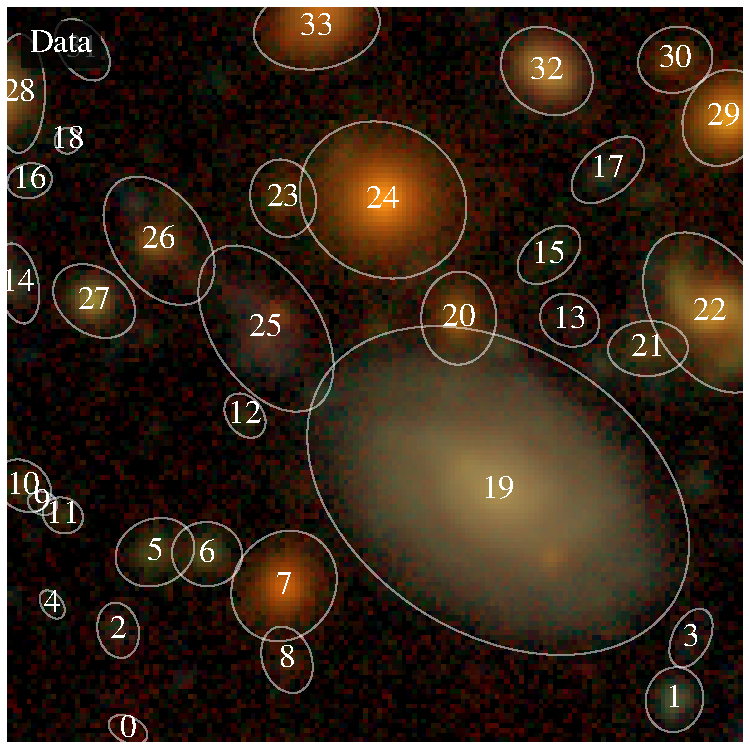
\includegraphics[width=.332\linewidth]{HSC_example_3_data}
    %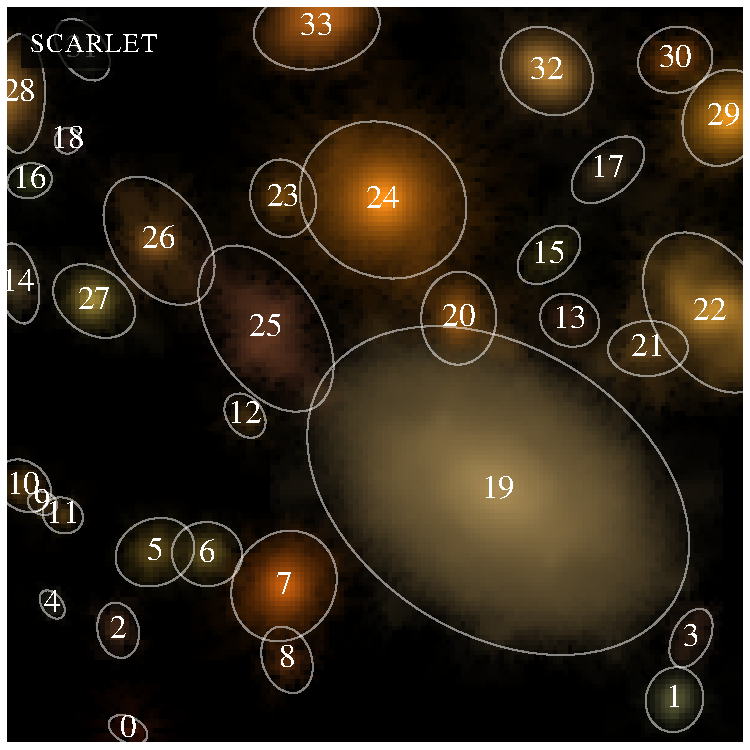
\includegraphics[width=.332\linewidth]{HSC_example_3_model}
    %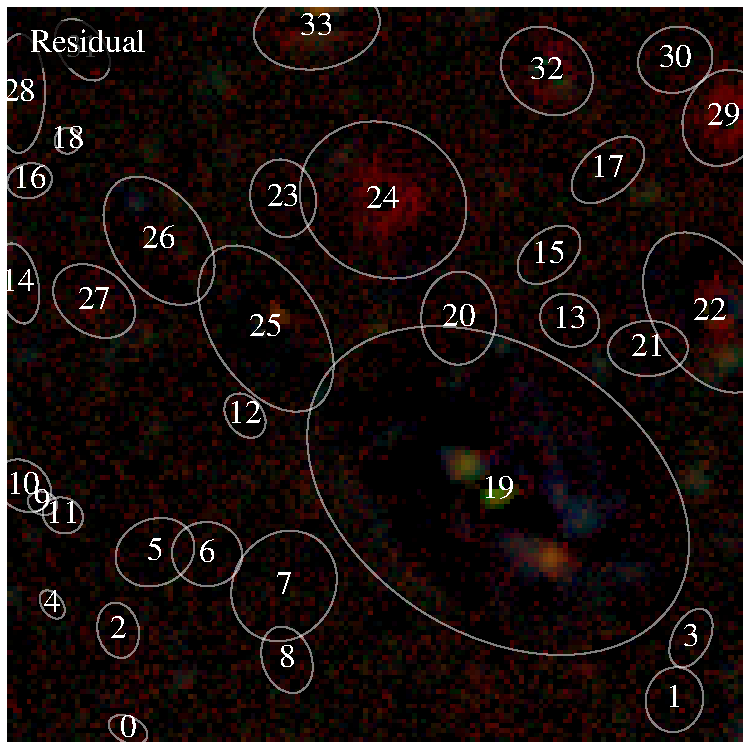
\includegraphics[width=.332\linewidth]{HSC_example_3_residual}

    \begin{center}
    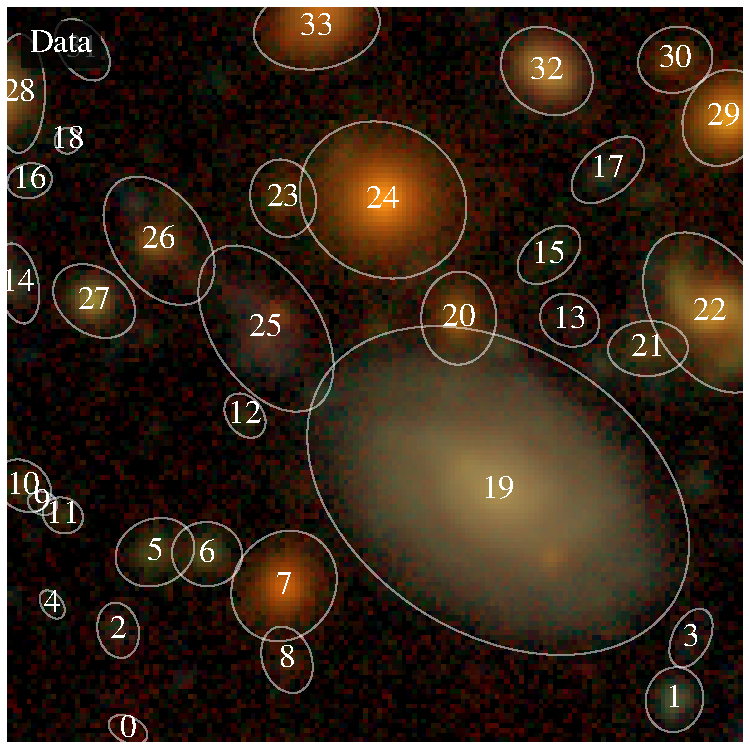
\includegraphics[width=.35\linewidth]{HSC_example_3_data}
    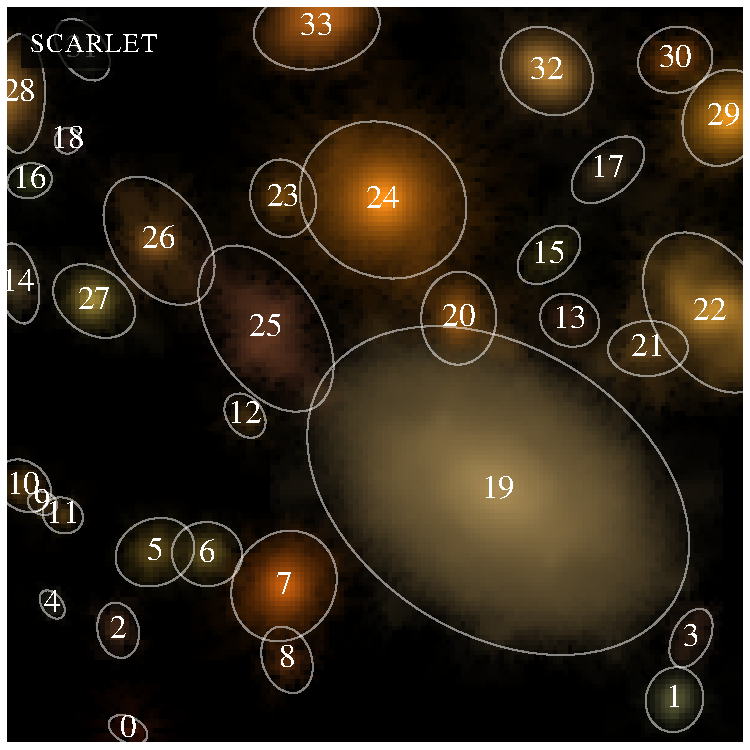
\includegraphics[width=.35\linewidth]{HSC_example_3_model}
    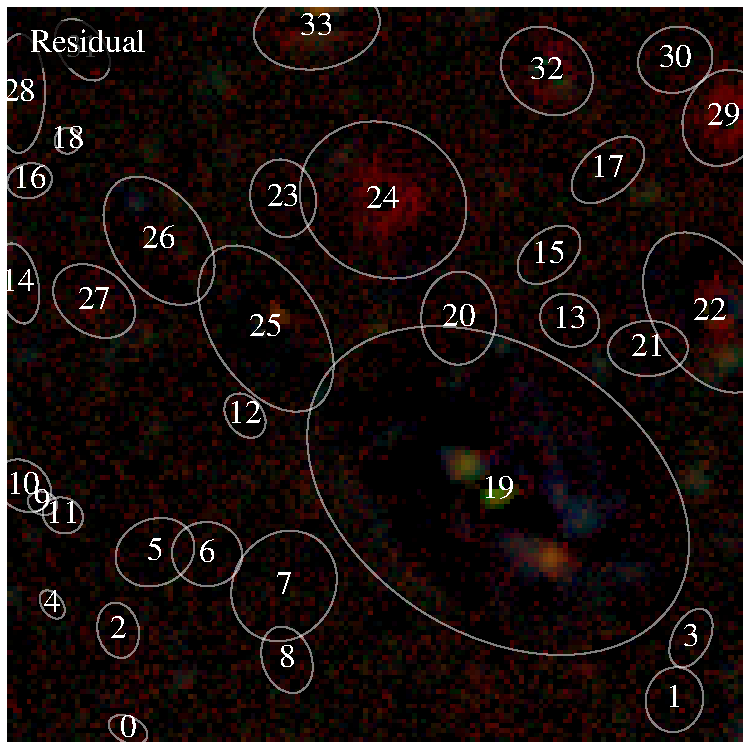
\includegraphics[width=.35\linewidth]{HSC_example_3_residual}
    \end{center}


}

\frame
{
    \frametitle{New MOF Deblender}

    \begin{itemize}

        \item See the previous talk by E. Sheldon.

    \end{itemize}

}



\frame
{
    \frametitle{Controlled Deblend Simulations}

    \begin{itemize}

        \item Simulate pairs of galaxies at various separations

        \item For what I will show, there is a ``central'' used
            to measure the shear.

        \item There is a ``neighbor'' which is twice as big and 33\% brighter.

        \item We have tried many models for these objects.  Shown here
            are examples for bulge+disk with knots of star formation.

        \item Unlike the new MOF model, the scale length of bulge and disk are
            different, they are not coelliptical or co-centric.  The knots follow
            the disk and can absorb up to 25\% of the disk flux.

    \end{itemize}

}
\frame
{
    \frametitle{Example MOF de-blended pair. Low Noise.}

    \includegraphics[width=0.9\linewidth]{{bdk-N0.1-r07-example}.png}

    Left is original, right is MOF deblended.
    \newline
    Can see residuals from ``knots'' of star formation.
}

\frame
{
    \frametitle{Example MOF de-blended pair. Medium Noise (S/N$\sim 50$.)}

    \includegraphics[width=0.9\linewidth]{{bdk-N10-r07-example}.png}

    Left is original, right is MOF deblended.

}

\frame
{
    \frametitle{Multiplicative bias $m$}

    \begin{center}
    \includegraphics[width=0.8\linewidth]{{bias_v_rad_mof_scar_bdk}.png}
    \end{center}


}

\frame
{
    \frametitle{Multiplicative bias $m$ (zoomed in)}

    \begin{center}
    \includegraphics[width=0.8\linewidth]{{bias_v_rad_mof_scar_bdk_zoom}.png}
    \end{center}


}
\frame
{
    \frametitle{Scarlet Problems}

    \begin{itemize}

        \item We have been working with Peter and Fred to improve the
            performance of Scarlet.

        \item Initially we were subtracting the model of the neighbor,
            but this didn't work well because the model absorbed
            some of the noise.  An accurate
            noise model is needed for \mcal\ and BFD.

        \item Currently using an SDSS-style ``two-step'' process that takes the
            models and reweights them to reproduce the observed image exactly.

        \item This is an improvement but not working as well as MOF yet,
            especially at high S/N.

    \end{itemize}

}


\frame
{
    \frametitle{Summary}

    \begin{itemize}
        \item New MOF unbiased in these sims at high S/N.

        \item New MOF shows separation-dependent biases, as expected, but
            approaches zero bias rapidly with increasing separation.

        \item Scarlet deblender results in a complex shear bias as 
            a function of separation.  Surprisingly worse at low
            noise.

        \item Scarlet deblender extremely flexible, clear improvement
            for large bright galaxies in dense fields.
            
        \item We don't know yet how best to use it in the regime most
            useful for shear: smallish faint galaxies

    \end{itemize}

}


\end{document}
